\documentclass[10pt]{article}
\newcommand {\ds} {\displaystyle}
\usepackage{color}
\usepackage{makeidx}
\usepackage{amsfonts}
\usepackage{fancyhdr}
\usepackage{multicol}

% --- Ajout pour TikZ ---
\usepackage{tikz}
\usetikzlibrary{arrows.meta}

\usepackage{amsmath, enumitem}
\usepackage[pass]{geometry}

%--------------------------------------------------------------------
\makeatletter
%                            \fillwithlines


% \fillwithlines takes one argument, which is either a length or \fill
% or \stretch{number}, and it fills that much vertical space with
% horizontal lines that run the length of the current line.  That is,
% they extend from the current left margin (which depends on whether
% we're in a question, part, subpart, or subsubpart) to the right
% margin.
%
% The distance between the lines is \linefillheight, whose default value
% is set with the command
%
% \setlength\linefillheight{.25in}
%
% This value can be changed by giving a new \setlength command.
%
% The thickness of the lines is \linefillthickness, whose default value
% is set with the command
%
% \setlength\linefillthickness{.1pt}
%
% This value can be changed by giving a new \setlength command.


\newlength\linefillheight
\newlength\linefillthickness
\setlength\linefillheight{.25in}
\setlength\linefillthickness{0.1pt}

\newcommand\linefill{\leavevmode
    \leaders\hrule height \linefillthickness \hfill\kern\z@}


\def\fillwithlines#1{%
  \begingroup
  \ifhmode
    \par
  \fi
  \hrule height \z@
  \nobreak
  \setbox0=\hbox to \hsize{\hskip \@totalleftmargin
          \vrule height \linefillheight depth \z@ width \z@
          \linefill}%
  % We use \cleaders (rather than \leaders) so that a given
  % vertical space will always produce the same number of lines
  % no matter where on the page it happens to start:
  \cleaders \copy0 \vskip #1 \hbox{}%
  \endgroup
}
\makeatother
%--------------------------------------------------------------------


\begin{document}

\begin{center}
$\phantom{}$\vspace{-1.5cm}\\
\rule{\linewidth}{1pt}\\
Universit\'{e} de Mayotte $\phantom{aa}$ D\'{e}partement Sciences et Technologies $\phantom{aa}$ 2026-2027 \\ \vspace{0.3cm}
  \textbf{   Contr\^{o}le terminal de "MG505 Combinatoire énumérative"  \\ L3 Math\'ematiques Générales  \\ Dur\'{e}e : 2 heures \\
   jeudi 12 novembre 2026 \\
(sans document, ni calculatrice, ni montre~\dots)}
\end{center}

\vspace{-0.3cm}
\rule{\linewidth}{1pt}

\textbf{Partie 1 : Théorie des graphes}

\textbf{Barème~:} $[0.5 + 1 + 1.5 + 1.5 + 1.5 + 1]$, $[0.5 + 1 + 1 + 1]$ et $[0.5 + 2]$

\vspace{0.1cm}
\textbf{Rappel.}
\begin{itemize}
  \item Les graphes considérés ici sont finis, simples et non orientés.
  \item L’ordre d’un graphe est le nombre de ses sommets.
\end{itemize}


\noindent \textbf{Exercice 1. Répondre sur une copie d'examen.}

Les six questions suivantes sont ind\'{e}pendantes.
\begin{enumerate}
\item Montrer que la séquence $S:=(1,1,1,1,1,1,1,1,2,2,2,3,3,4)$ n'est pas la séquence de degrés d'un graphe connexe.

\item Montrer qu'il n'existe aucun graphe $G:=(V,E)$ tel que~:
$$|V|=11, \quad |E|=26, \quad \text{et } (\forall x \in V, \ d_G(x) \in \{3,8\}).$$

\item Soit $T$ un arbre d'ordre $n \geq 2$.\\
Montrer que si $T$ admet exactement $2$ feuilles, alors $T$ est un chemin.

\item Soit $T$ un arbre d'ordre $n \geq 3$, et soit $\overline{T}$ son graphe complémentaire.\\
Montrer que si $T$ n'est pas une étoile, alors $\overline{T}$ est connexe.

\item Pour chacun des deux graphes bipartis complets $K_{4,2026}$  et $K_{2027,2027}$, indiquez s'il est eulérien, s'il est semi-eulérien et s'il est hamiltonien. \\
    Justifiez brièvement vos réponses.

\item Déterminer tous les entiers $p, q \geq 1$ pour lesquels le graphe biparti complet $K_{p,q}$ est planaire.
\end{enumerate}

\newpage
\noindent \textbf{Exercice 2. Répondre sur une copie d'examen.}

Considérons le graphe $G$ représenté ci-dessous :

\begin{center}
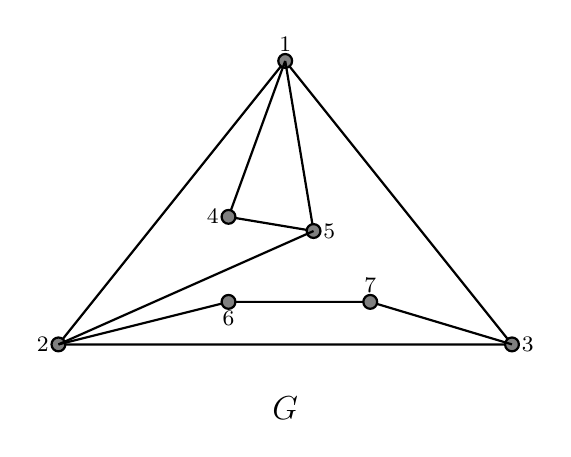
\begin{tikzpicture}[scale=0.36,font=\footnotesize]
 \tikzstyle{sommet}=[circle, draw, fill=black!50, inner sep=0pt, minimum width=5pt]

% Étiquettes des sommets
\node   at (0,10)   [above]  {$1$};
\node   at (-8,0)   [left]   {$2$};
\node   at (8,0)    [right]  {$3$};
\node   at (-2,4.5) [left]   {$4$};
\node   at (1,4)    [right]  {$5$};
\node   at (-2,1.5) [below]  {$6$};
\node   at (3,1.5)  [above]  {$7$};

\node   at (0,-1.5) [below]  {\large{$G$}};

% Triangle extérieur 1--2--3
\draw [thick] (0,10) node[sommet]{} --(-8,0) node[sommet]{} --(8,0) node[sommet]{} --(0,10);

% Arêtes intérieures
\draw [thick] (0,10) -- (-2,4.5) node[sommet]{} -- (1,4) node[sommet]{} -- (0,10);   % 1--4, 4--5, 5--1
\draw [thick] (1,4) -- (-8,0);                                                      % 5--2
\draw [thick] (-8,0) -- (-2,1.5) node[sommet]{} -- (3,1.5) node[sommet]{} -- (8,0);   % 2--6, 6--7, 7--3

\end{tikzpicture}
\end{center}

 \begin{enumerate}
 \item Le graphe $G$ est-il eulérien ? Si oui, en donner un tour eulérien.
 \item Le graphe $G$ est-il semi-eulérien ? Si oui, en donner un parcours eulérien.
\item Montrer que le graphe $G$ est hamiltonien.
\item Montrer que le graphe $G - e$, obtenu à partir de $G$ par suppression de l'arête $e = \{2,5\}$, est non hamiltonien.

\end{enumerate}

\noindent \textbf{Exercice 3. Répondre sur une copie d'examen.}

Le département de mathématiques d'une universit\'e doit organiser les
horaires des examens. On
suppose qu'il y a 7 \'epreuves \`a planifier, correspondant aux
cours num\'erot\'es de 1 \`a 7 et que les paires de cours ayant
des \'etudiants en commun sont : $\{1, 2\}$, $\{1, 3\}$, $\{1, 5\}$, $\{2, 3\}$, $\{2, 4\}$,
$\{2, 6\}$, $\{3, 5\}$, $\{3, 7\}$, $\{4, 6\}$,
$\{4,7\}$, $\{5, 6\}$ et $\{6, 7\}$.

On cherche une organisation de ces examens sur une dur\'ee minimale
(un \'etudiant ne pouvant pas passer deux \'epreuves en m\^eme
temps).
\begin{enumerate}
\item Représenter cette situation par un graphe $G$, dont on précisera les sommets et les arêtes.
\item Déterminer le nombre chromatique $\chi(G)$ du graphe $G$. En déduire une organisation de ces examens sur une durée minimale.
\end{enumerate}

\newpage

\begin{center}
$\phantom{}$\vspace{-1.5cm}\\
\rule{\linewidth}{1pt}\\
Universit\'{e} de Mayotte $\phantom{aa}$ D\'{e}partement Sciences et Technologies $\phantom{aa}$ 2026-2027 \\ \vspace{0.3cm}
  \textbf{   Contr\^{o}le terminal de "MG505 Combinatoire énumérative"  \\ L3 Math\'ematiques Générales  \\ Dur\'{e}e : 2 heures \\
   jeudi 12 novembre 2026 \\
(sans document, ni calculatrice, ni montre~\dots)}
\end{center}

\vspace{-0.3cm}
\rule{\linewidth}{1pt}

\textbf{Partie 2 : Théorie des nombres}

\textbf{Barème~:} $[7]$


\noindent \textbf{Exercice 4. Répondre sur le sujet ci-dessous.}

	Benjamin joue à un jeu avec les lumières de la cathédrale de Clermont-Ferrand.
	
	Il dispose de 1000 interrupteurs numérotés de 1 à 1000.
	Lorsque actionné, un interrupteur change d'état : il passe d'allumé à éteint, ou d'éteint à allumé.
	Au départ, tous les interrupteurs sont éteints.
	
	Benjamin actionne successivement les interrupteurs comme suit :
	\begin{enumerate}[align=right, leftmargin=60pt]
		\item
		tous les multiples de 1 sont actionnés ; puis
		\item
		tous les multiples de 2 sont actionnés ; puis
		\item
		tous les multiples de 3 sont actionnés ; puis
		\item[$\vdots$]
		\item[999.]
		tous les multiples de 999 sont actionnés ; et enfin
		\item[1000.]
		tous les multiples de 1000 sont actionnés.
	\end{enumerate}
	À la fin du jeu, quels interrupteurs sont allumés et quels interrupteurs sont éteints ?
	
	\emph{Toute trace de recherche sera prise en compte.}

\noindent \textbf{Réponse à l'exercice 4.}

\fillwithlines{7cm}

\newpage
\newgeometry{
	margin=2cm,
	right=2.2cm,
	footskip=1.5cm,
}

\noindent \textbf{Réponse à l'exercice 4.}

\fillwithlines{22cm}

	
	
\end{document}

